\documentclass[a4paper,12pt]{article}
\usepackage[english]{babel}
\usepackage[utf8]{inputenc}
\usepackage{fontspec}
\setmainfont{CMU Serif}

\newfontfamily{\englishfont}{CMU Serif}
\newfontfamily{\thaifont}[Scale=MatchUppercase]{TH Sarabun Chula}
\newenvironment{thailang}{\thaifont}

\usepackage[Latin,Thai]{ucharclasses}
\setTransitionTo{Thai}{\thaifont}
\setTransitionFrom{Thai}{\englishfont}

\XeTeXlinebreaklocale "th_TH"
\XeTeXlinebreakskip = 0pt plus 1pt 

\usepackage{setspace}
\onehalfspacing

\usepackage{amsmath,amsthm,amssymb}
\usepackage{physics}
\usepackage[margin=1in]{geometry}

\usepackage{graphicx}

\begin{document}
		\begin{center}
			\large\textbf{ข้อสอบ สอวน. ม.5 ศูนย์โรงเรียนเตรียมอุดมศึกษา ค่ายเดือนมีนาคม 2558}\\
			\normalsize จัดพิมพ์ใหม่โดย Ittipat
		\end{center}

\section{เหรียญกลิ้งในกรวย}
เหรียญกลมมวล $M$ และรัศมี $r$ กลิ้งโดยไม่ไถลภายในกรวยที่ยึดอยู่ที่กับที่ โดยที่ระนาบการหมุนของเหรียญตั้งฉากกับผิวของกรวย ให้ลูกบอลเคลื่อนที่ในระนาบที่ขนานกับแนวราบที่สูงจากปลายกรวย $h$ โดย $r\ll h\tan\theta$ แกนกรวยตั้งฉากกับแนวระนาบและมุมปลายกรวยเท่ากับ $2\theta$ ให้ความเร่งโน้มถ่วงเป็น $g$
	\begin{figure}[h]
	\centering
	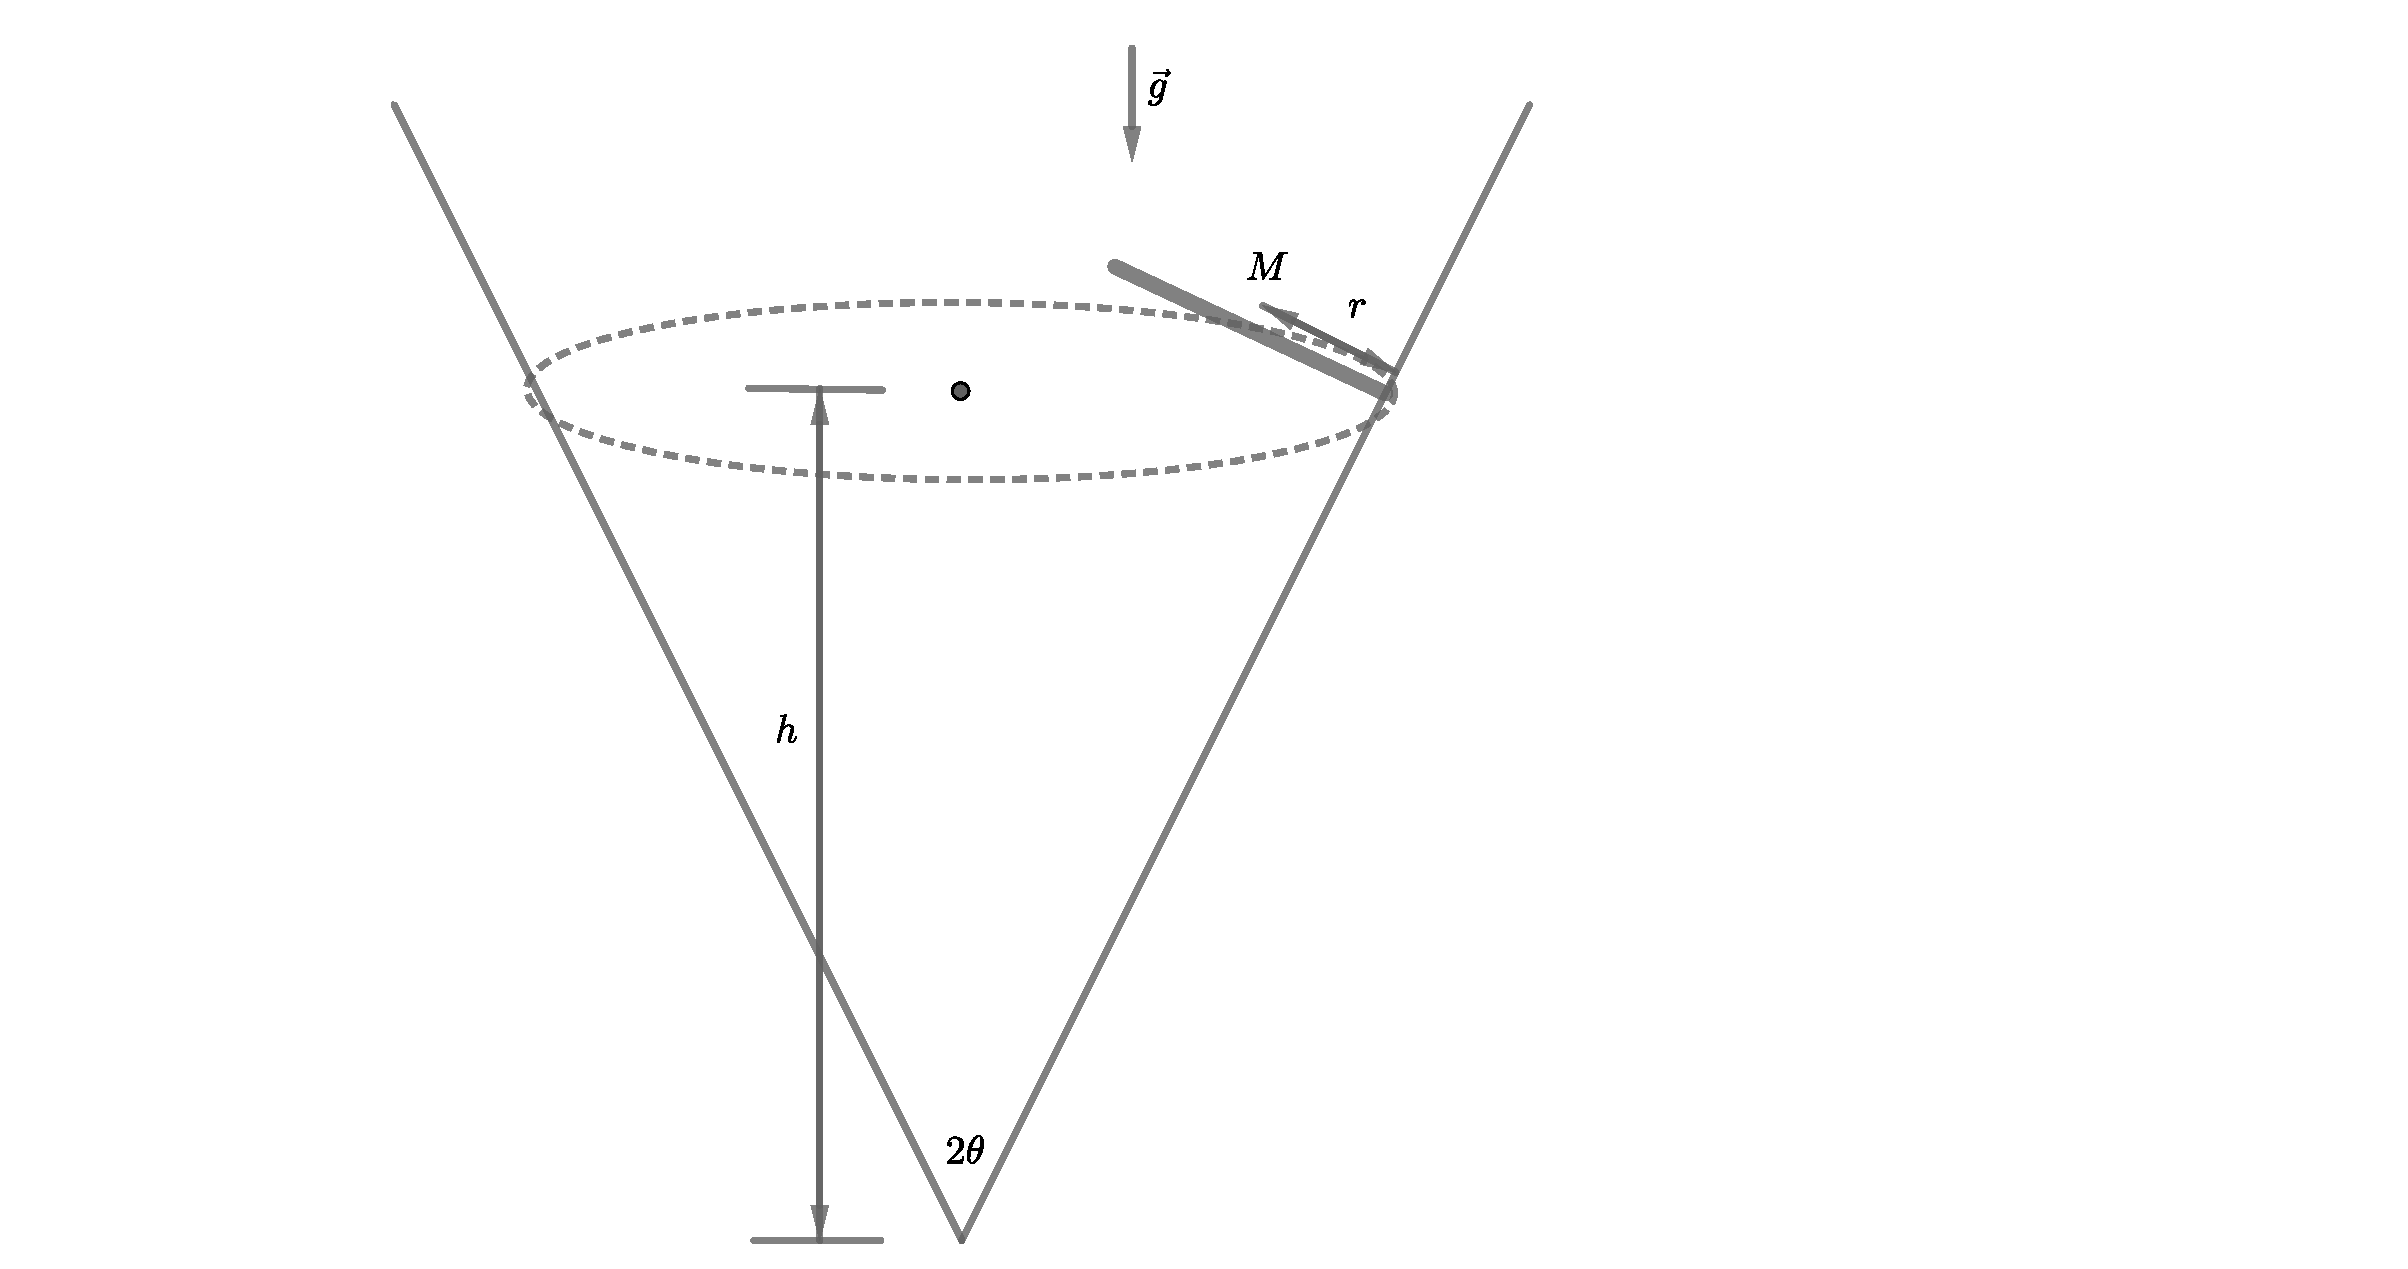
\includegraphics[scale=0.4]{1}
	\label{fig:1}
	\end{figure}
\\ก. จงหาความเร็วเชิงมุม $\vec{\Omega}$ ที่เหรียญเคลื่อนที่เป็นวงกลมรอบแกนกรวย \hfill(5 คะแนน)\\
ข. หาโมเมนตัมเชิงมุมรวมของเหรียญ $\vec{L}_{tot}$ (แนะนำ นักเรียนต้องรวมโมเมนตัมเชิงมุมจากการที่เหรียญเคลื่อนที่เป็นวงกลมรัศมี $R$ ด้วย และ ควรใช้ระบบพิกัดเชิงขั้ว (polar coordinate)\\(5 คะแนน)

\section{ลูกตุ้มบนโต๊ะหมุน}
ลูกตุ้มมวล $M$ ยึดติดกับคานที่วางบนเสา 2 ข้าง โดยที่เสาถูกยึดกับพื้นของโต๊ะกลมที่หมุนด้วยความเร็วเชิงมุม $\Omega$ ดังแสดงในรูป ให้แท่งที่ยึดลูกตุ้มอยู่กับคาน ยาว $l$ และมีมวลน้อยมากๆ จนไม่ต้องคำนึงถึง ให้ความเร่งโน้มถ่วงเป็น $g$ และไม่ต้องคำนึงถึงการหมุนของโลก ให้คานกับแท่งที่ยื่นไปยึดกับลูกตุ้มเป็นวัตถุชิ้นเดียวกัน และหมุนด้วยความเร็วเชิงมุม $\Omega$ ไปพร้อมกับโต๊ะ
\pagebreak
	\begin{figure}[h]
	\centering
	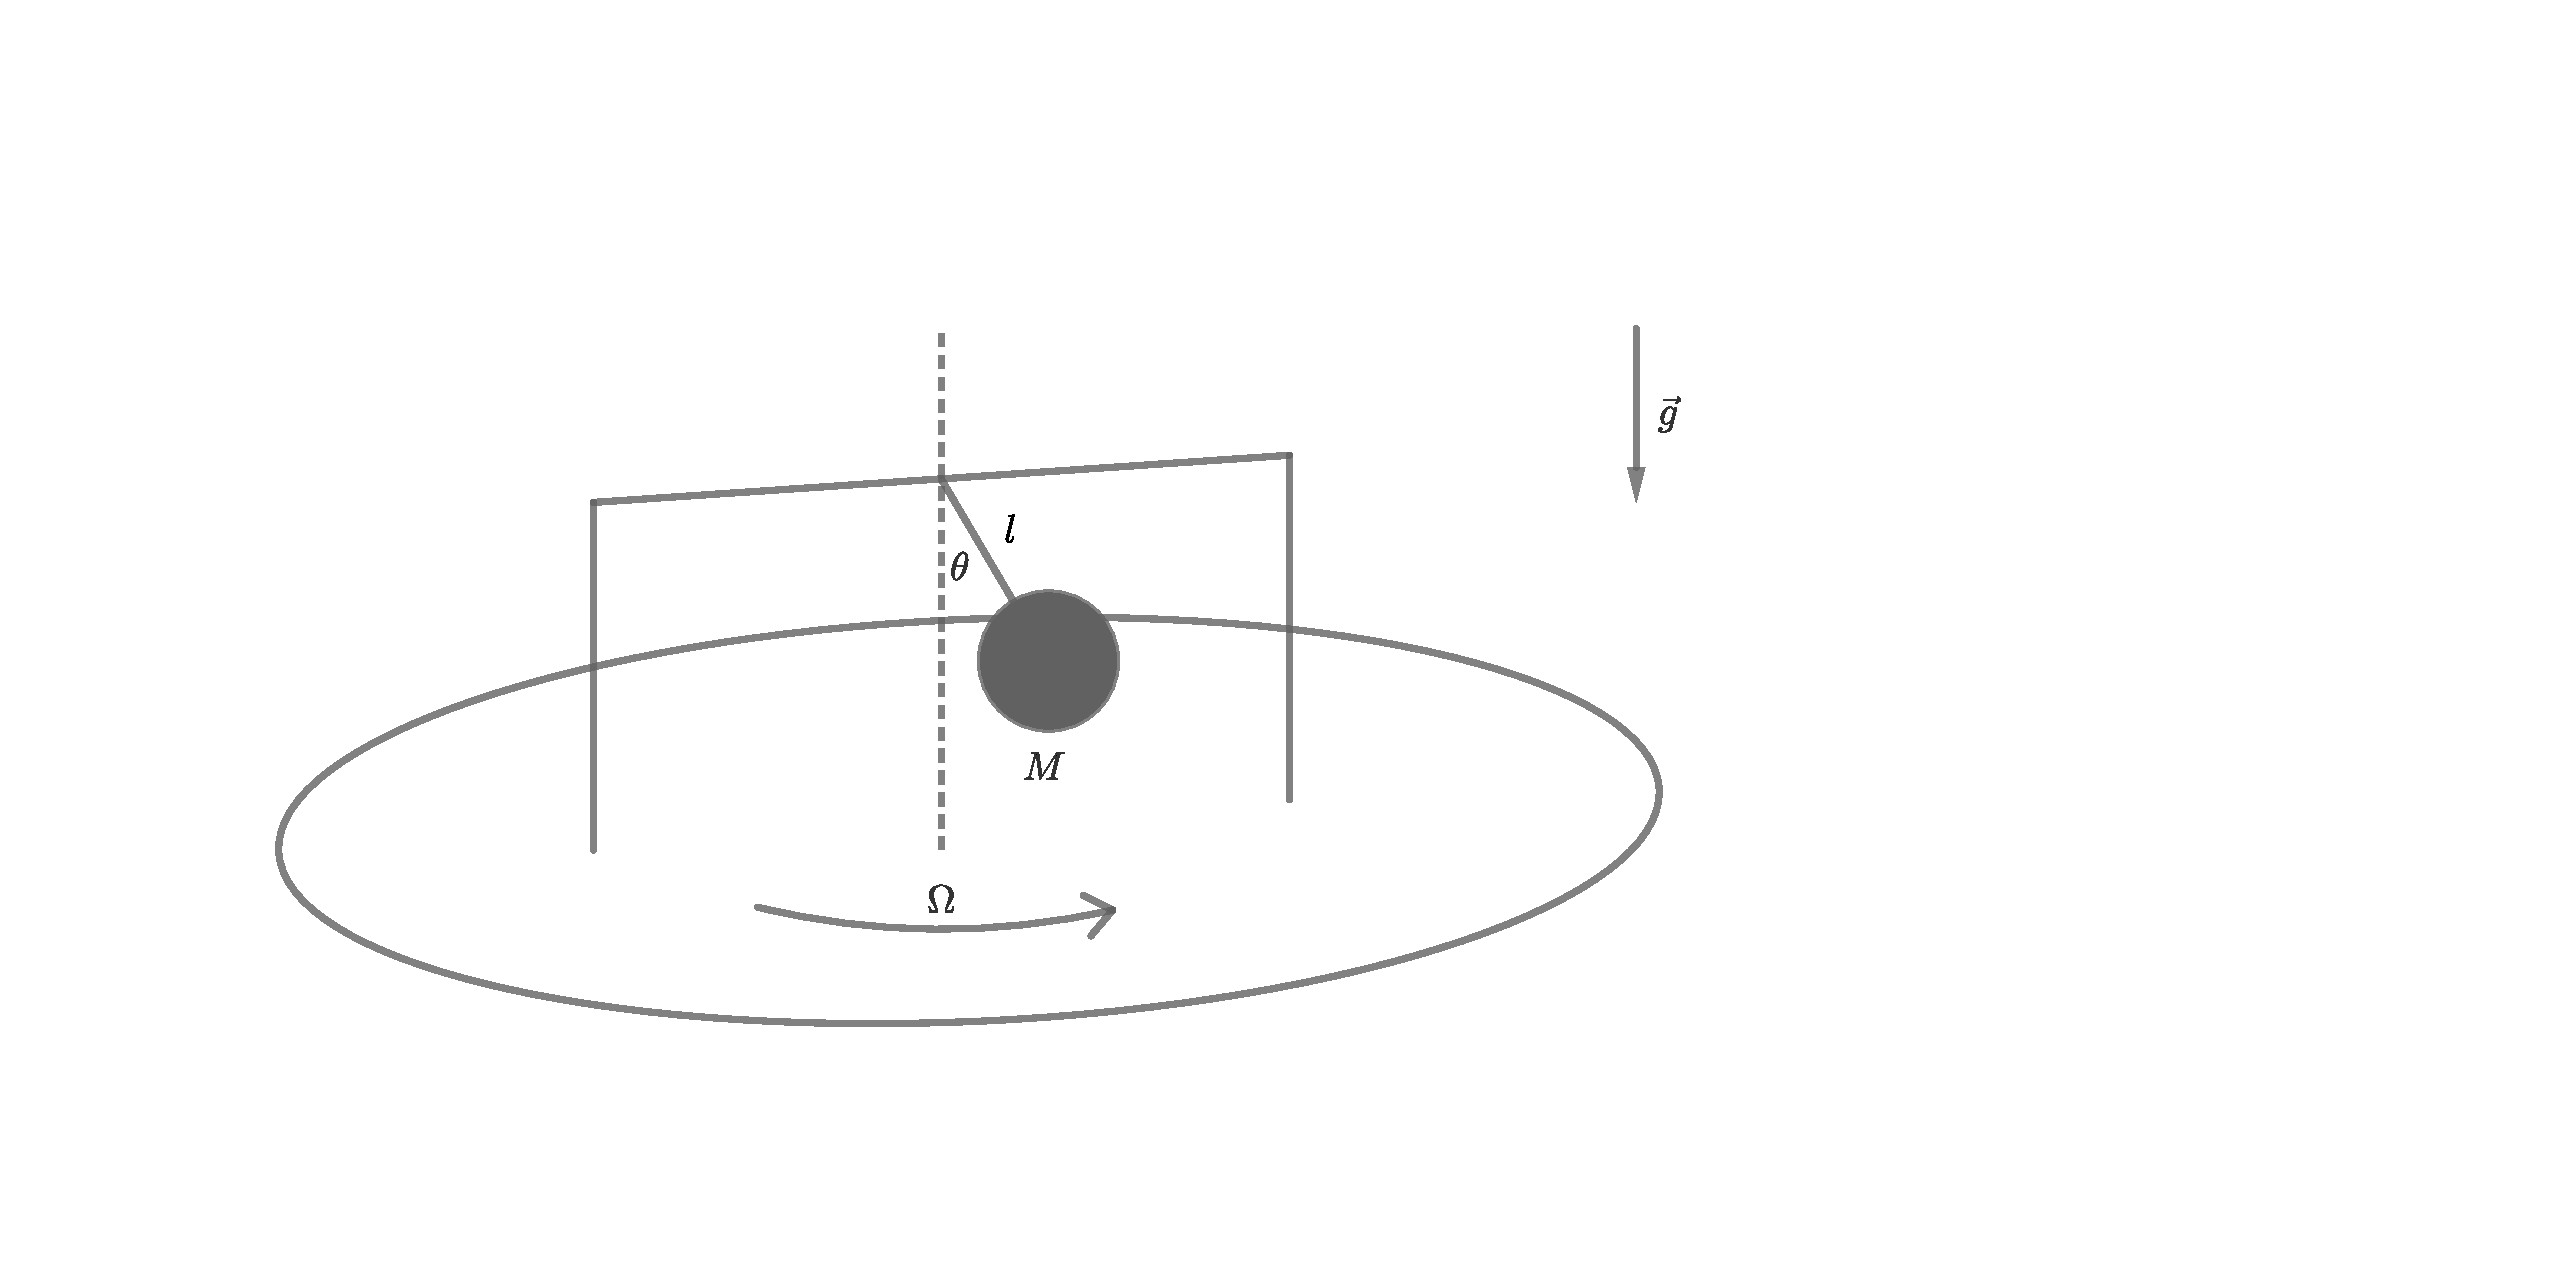
\includegraphics[scale=0.4]{2}
	\label{fig:2}
	\end{figure}
\\ก. หาสมการการเคลื่อนที่ของมวลในกรอบอ้างอิงของโต๊ะที่หมุน ในข้อนี้นักเรียนไม่ต้องใช้การประมาณมุม $\theta$ เล็กๆ และให้เขียนสมการในระบบพิกัดเชิงขั้ว\hfill(5 คะแนน)\\
ข. หาคาบการแกว่งของลูกตุ้ม ให้ใช้การประมาณมุม $\theta$ เล็กๆ\hfill(5 คะแนน)
\end{document}
	